%!TEX root = ../Base.tex

\chapter{Metodología}

\epigraphhead[70]{
\epigraph{``Data! Data! Data!'' he cried impatiently. 
``I can't make bricks without clay.''}{Sherlock Holmes}}

\section{Esquema general} 

Agregar esquema de la metodología que se siguió.

\section{Resolver modelo HMM usando EM} 
\label{sec:sd-hmm-em}

Para las pruebas que se han realizado hasta ahora, se han usado grabaciones creadas sintéticamente; esto es, usando un sintetizador de voz. El hacer las grabaciones con voces sintéticas nos permite tener un mayor control sobre la calidad de la grabación (no hay ruidos aditivos o interferencias), además de poder generar muchos más casos de prueba sin tantas complicaciones.

Para las primeras pruebas, se utilizó una grabación correspondiente a varios poemas de la autoría de Manuel Acuña, recitados por varios interlocutores.

Mediante bootstrap se busca genera un modelo representativo para cada una de las propuestas, y  se hace la elección del número correcto de speakers identificados mediande BIC.

Para las pruebas, se analizaron modelos desde 2 hasta 7 personas participantes, mientras que los resultados que se prensentan son las segmentaciones obtenidas usando desde 2 hasta 4 speakers; además de comparar el ground truth.

\begin{comment}
\begin{figure}[bth]
  \centerline
  {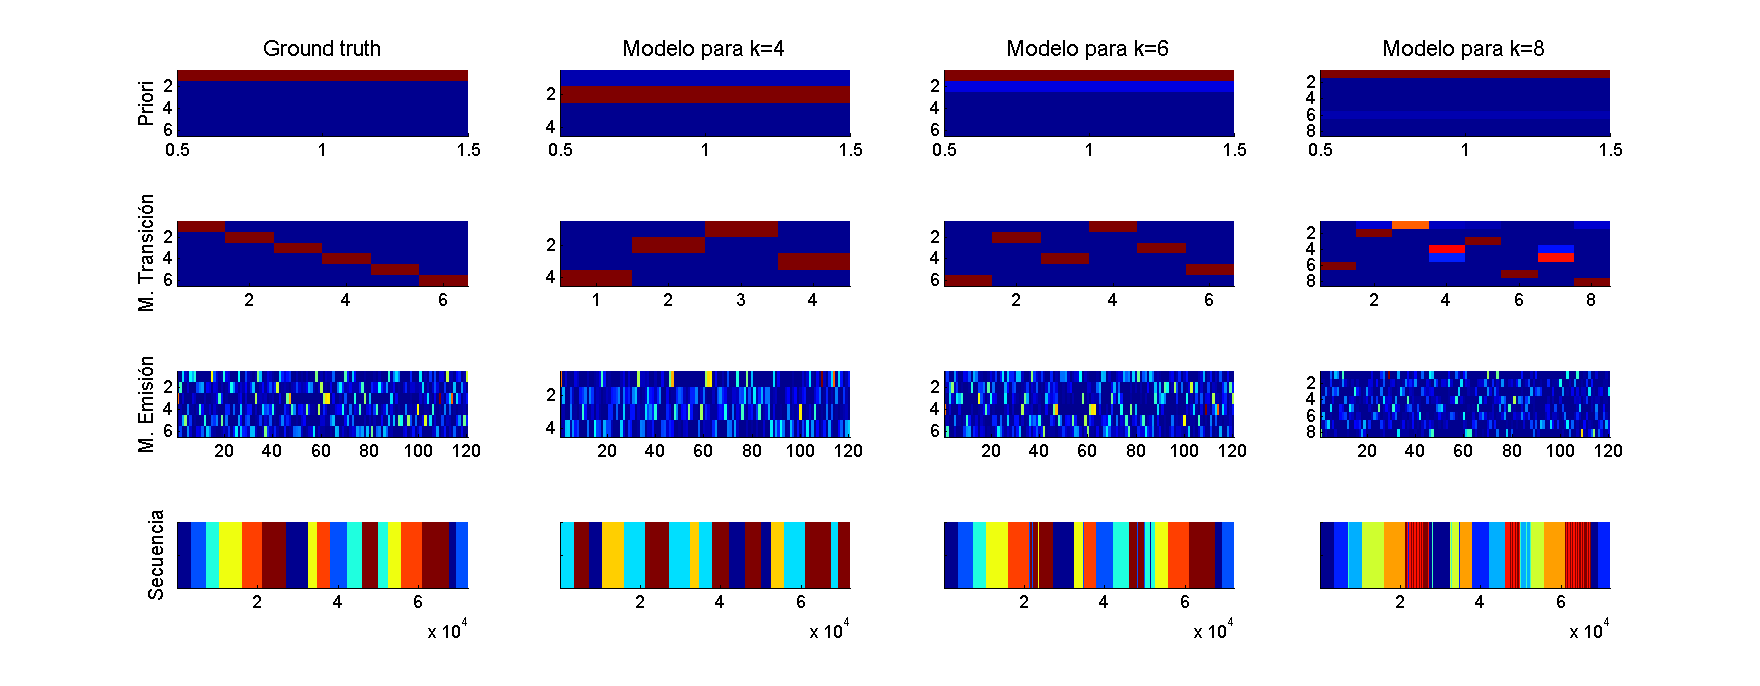
\includegraphics[width=1.7\linewidth]{gfx/chap5/cuerv-1}} \quad
  \caption{Parámetros estimados para Prueba 1}
  \label{fig:cald-1}
\end{figure}
\end{comment}

En la \autoref{fig:cald-1} se muestran los parámetros estimadosa a forma de matrices en falso color: la matriz inicial o a priori, la matriz de transiciones entre speakers, la matriz de emisión de cada speaker para todo el diccionario de palabras, así como la secuencia recuperada.

Como ya se había mencionado, hay un problema de identificación con los interlocutores, por lo que en muchos casos las matrices no corresponderán tal cual, sino que puede que haya intercambio entre las personas que se identificaron.

A partir de esto, y dependiendo de que la segmentación sea confiable, se puede usar algún algoritmo para deducir y emparejar a cada uno de los speakers detectados con su correspondiente en el ground truth.

Se muestra esta comparación, en tanto en \autoref{fig:cald-21} como en \autoref{fig:cald-22}. Las secuencias recuperadas se representan como series de tiempo en donde además se marcan en rojo los errores al asignar a una persona equivocada.

Se puede observar como para el caso en que el modelo se ajusta para 3 personas, la secuencia recuperada en escencia es la misma, exceptuando algunos saltos que se presentan a veces; pero en general logra detectar de forma correcta cada que hay un cambio de interlocutor en la grabación original.

\begin{comment}

\begin{figure}[bth]
  \centerline
  {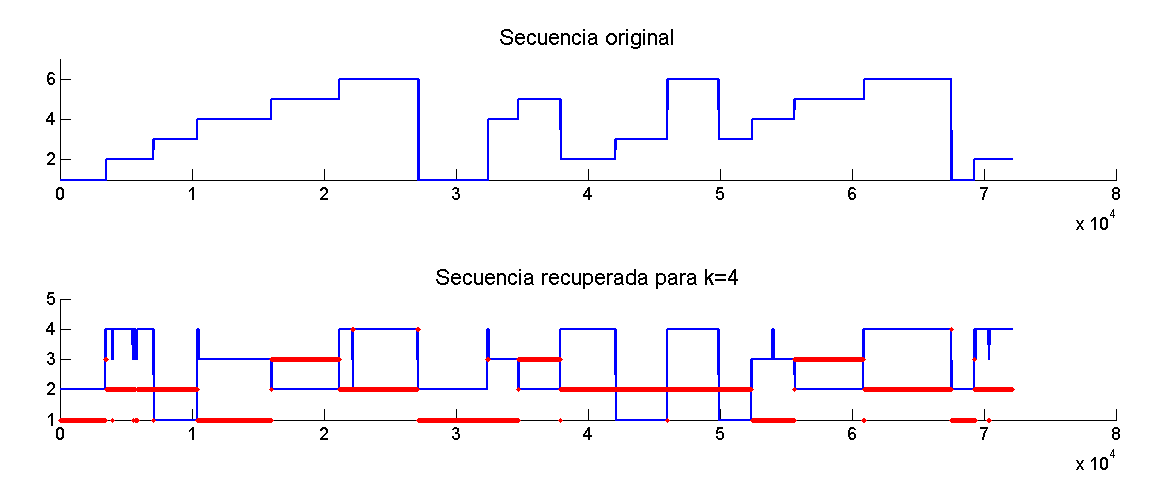
\includegraphics[width=1.5\linewidth]{gfx/chap5/cuerv-21}} \quad
  \caption{Secuencia recuperada para Prueba 1}
  \label{fig:cald-21}
\end{figure}

\begin{figure}[bth]
  \centerline
  {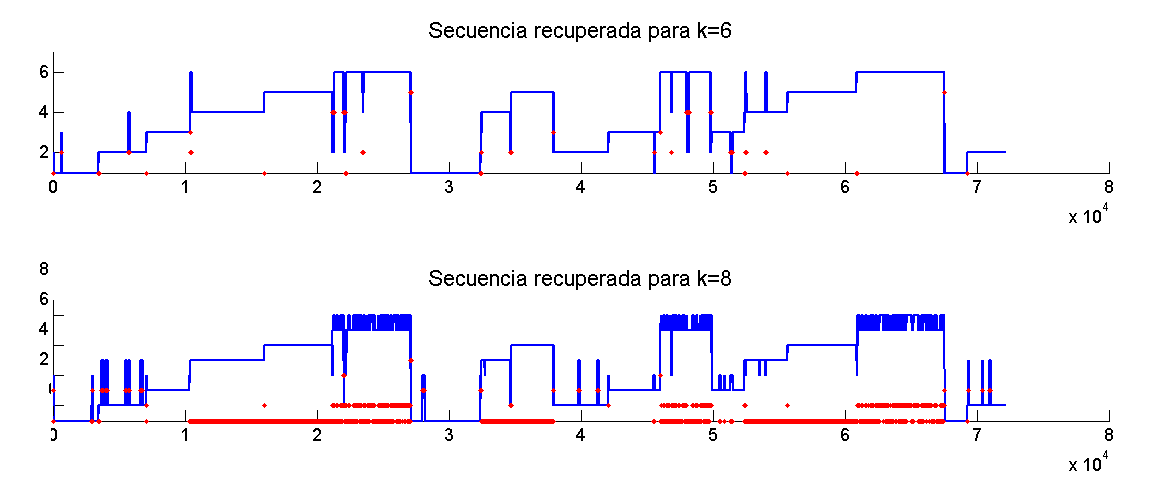
\includegraphics[width=1.5\linewidth]{gfx/chap5/cuerv-22}} \quad
  \caption{Secuencia recuperada para Prueba 1}
  \label{fig:cald-22}
\end{figure}

\end{comment}

Ahora, al usar BIC para la selección del modelo, obtenemos la siguiente gráfica, con la que se observa que el modelo que se ajusta de mejor manera es en efecto el correspondiente a 6 personas, como se puede observar en la gráfica 

\begin{comment}
\begin{figure}[bth]
  \centerline
  {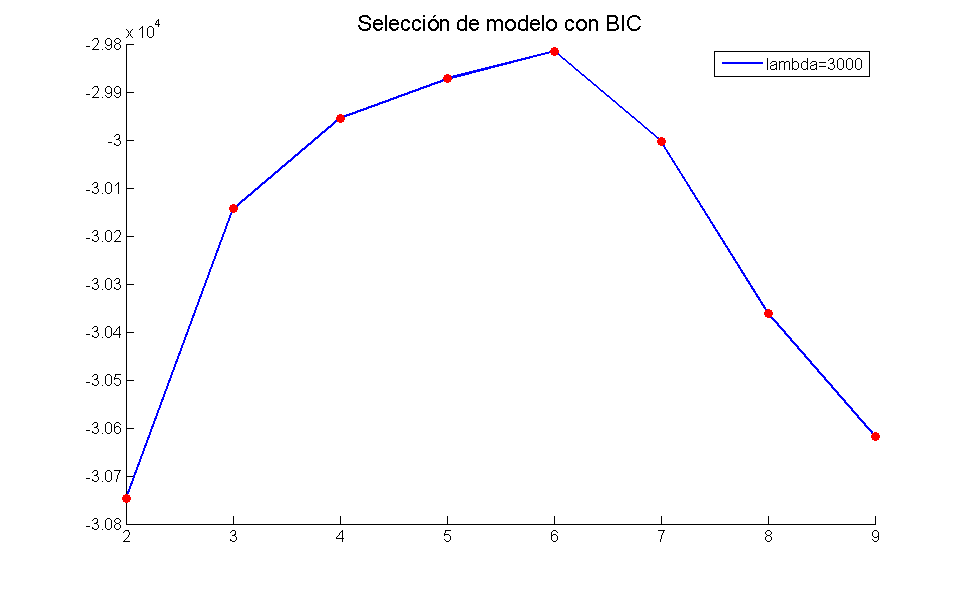
\includegraphics[width=0.9\linewidth]{gfx/chap5/cuerv-0}} \quad
  \caption{Selección de modelo usando BIC}
  \label{fig:cald-0}
\end{figure}
\end{comment}

Para la segunda prueba, se utilizon varias composiciones del escritor Edgar Allan Poe, que fueron generadas de la misma manera sintéticamente, pero ahora utilizando un motor de voz en inglés.

Se muestran a continuación los resultados obtenidos de la misma manera.

En estas gráficas se observa de igual manera cómo se logró estimar de forma correcta el número de interlocutores. Cuando se aplica el modelo para un número menor que el real, se detectan las inconsistencias y aumenta la tasa de error; así como cuando se ajusta el modelo para un número mayor de personas, se sobreajusta el modelo y se marcan como errores.

